
The global ledger state is stored locally by each node in a key value pair database. Any performant database such as RockDb can be used to store the state data, however the data must be organised using a structure called a Sparse Merkle Tree. This structure allows the entire data state to be represented by a single hash, known as the root hash. Any changes to the data would result in a completely different root hash, therefore it can be used by nodes to verify that their dataset is the same as that of other nodes. Consequently, a node using an alternative storage organisation would be unable to interact with the network due to an inability to calculate the same root hash.\\

The Sparse Merkle Tree data structure allows for:

\begin{enumerate}
\item Persistent storage of the current and previous states of the ledger.
\item Efficient provision of proof that queried data exists, or importantly, does not exist in the ledger.\end{enumerate}

In addition to storing the global ledger state in a Sparse Merkle Tree, the smart contract KVM code and smart contract data are also stored as a Sparse Merkle Tree. This allows the root hash of both these data sets to be stored in the \textbf{storageRoot} and \textbf{codeHash} fields in the account state.  The use of the SMT for storing these data sets allows honest nodes to recognise and reject information that has been altered outside of the ledger cycle by malicious parties. \\

\subsubsection{Merkle Tree}

Each item of data being stored (here the serialised account information) is represented as a leaf of the Merkle tree. The data in neighbouring leaves is hashed and concatenated and this value is used for the node one level above in the tree. Each node is stored in the database with its lookup key being the hash of its value. Every leaf node is labelled with the hash of a data block, and every non-leaf node is labelled with the cryptographic hash of the labels of its child nodes. The nodes are themselves combined until a single hash has been obtained. This is the root hash and its value depends on every bit of data stored in the tree.\\

\begin{figure}[h]
  \centering
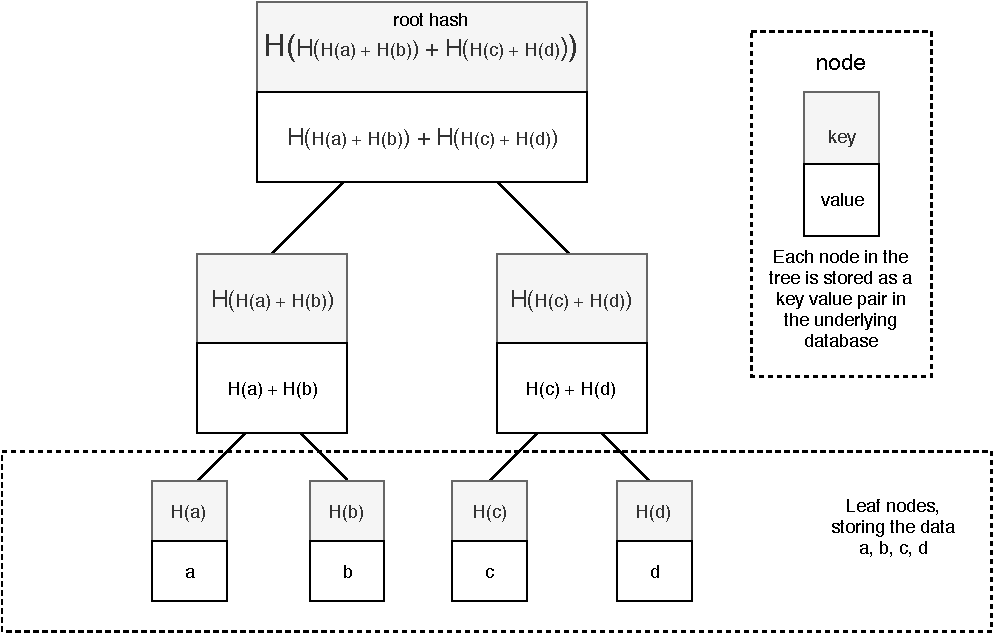
\includegraphics[scale=0.8]{merkle-tree}
\end{figure}

When a data entry changes, every node above it in the tree must be recalculated. The hash of the data held by a node is used as its key in the database, therefore every recalculated node will constitute a new entry in the underlying database, rather than an existing entry that needs to be updated.\\

\subsubsection{Merkle Proof}

A client with knowledge of the current root hash of the state tree does not need to retrieve the complete set of data to verify the inclusion of a specific entry. Knowledge of each sibling hash along the path down to the entry being authenticated is sufficient to reconstruct the root hash. A client who is able to reconstruct the root hash from this data can be confident that the entry is contained in the data set. For example, in the diagram above, the inclusion of entry \textbf{a} can be verified with just \textbf{a}, \textbf{H(A)}, and \textbf{H(c)+H(d)}. 

Though it is simple to prove inclusion of an item using many different kinds of Merkle Tree, proving that a particular item is \emph{not} included can be harder. Where the leaf node 

\subsubsection{Sparse Merkle Tree}

The Sparse Merkle Tree

To store or retrieve an entry from a Merkle trie, a key is used. For the account storage we use the account address as the key. This key is not equivalent to a key in the underlying database, instead it is used to determine the path from the root hash to the data entry. The key tells us which branch to follow as we progress down the tree.  

\begin{figure}[h]
  \centering
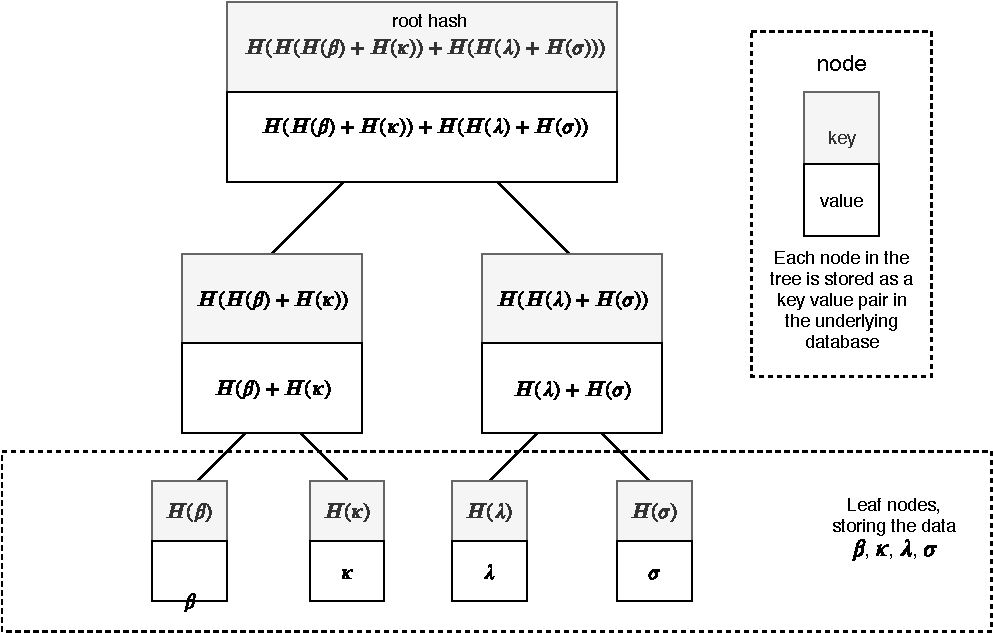
\includegraphics[scale=0.8]{sparse-merkle-tree}
\end{figure}


\subsubsection{Choice of Sparse Merkle Tree over Merkle Patricia Tree}

Using a binary tree gives us very simple and easy to use Merkle proofs. In a Patricia tree, a Merkle proof is composed of all the nodes in the path of a key. Since each node has 16 children the quantity of data is larger and not as straightforward to verify as in binary.
The sparse Merkle tree also provides convenient proofs of non-inclusion: the proof that a key is not included in the tree is simply a proof that the value for the key is default .

-balanced
-easy proof of non existence
-simpler to implement

